\documentclass[12pt]{article}
\usepackage[hmargin=0.75in, vmargin=1in]{geometry}
\geometry{letterpaper}
\usepackage[T1]{fontenc} 
\usepackage[utf8]{inputenc} 
\usepackage[french]{babel}
\usepackage{graphicx} % Support for including images
\usepackage{hyperref} % Support for hyperlinks
\hypersetup{hidelinks = true}
\usepackage{amsmath}
\usepackage{amssymb}
\usepackage{siunitx}
\usepackage{xcolor}
\sisetup{
    round-mode = figures,
    round-precision    = 3           ,
    scientific-notation = true
    }
\usepackage{float}
\usepackage{cancel}
\usepackage{tikz}
\usepackage{booktabs}
\usepackage{comment} 
\usepackage{minted}
\renewcommand{\thesection}{\arabic{section}}
\newcommand*{\rttensor}[1]{\bar{\bar{#1}}}
\newcommand*\circled[1]{\tikz[baseline=(char.base)]{
            \node[shape=circle,draw,inner sep=2pt] (char) {#1};}}
\newcommand{\pder}[2][]{\frac{\partial#1}{\partial#2}}
%------------------------------------------------------------------
% TITLE
%------------------------------------------------------------------
\title{
\centerline{
\includegraphics[width=0.4\textwidth]{images/poly}}
\vspace{0.5 cm}
Projet \\
\vspace{1cm}
ENE6002
\large  \\
Thermohydraulique des systèmes diphasiques \\ 
\Huge-\\
\normalsize Polytechnique Montréal
  }

\author{
    \begin{minipage}{.46\textwidth}
        \begin{center}
            Thomas \textsc{Charpentier} - 2036024\\
            \texttt{thomas.charpentier@polymtl.ca}
        \end{center}
    \end{minipage}%
    \hfill\vrule\hfill
    \begin{minipage}{0.46\textwidth}
        \begin{center}
            Gaétan \textsc{Raynaud} - 2022063\\
            \texttt{gaetan.raynaud@polymtl.ca}
        \end{center}
    \end{minipage}
}    

\date{\today}


%------------------------------------------------------------------
% DOCUMENT START HERE
%------------------------------------------------------------------
\begin{document}
\maketitle
\tableofcontents
\newpage
\section{Introduction et présentation de l'étude\label{section:pres}}

\subsection{Introduction}

Dans les applications industrielles, dès lors que l'on travaille avec un écoulement dans un conduite chauffée, on peut observer en parallèle de la phase liquide l'apparition de vapeur. Entre ces deux phases il s'échange de la masse, de l'énergie et de la quantité de mouvement et le désordre généré s'accompagne généralement d'une chute de pression. Si la conduite est suffisamment longue, la prise en compte des pertes de charges dans un modèle monophasique risque d'être peu représentatif de la réalité, les pertes liées à l'ébullition n'étant pas négligeables.\\

Cette sous-estimation de la perte de pression lors du dimensionnement peut avoir des répercussions sur le rendement de l'installation ou bien sa sécurité. Dans le cas d'un réacteur à eau pressurisé, il est important de connaître les conditions de l'écoulement à tous les endroits de la conduite. On ne souhaite pas se retrouver avec un écoulement diphasique dans une zone où cela n'était pas prévu, avec des conséquences majeures pour la sécurité. De plus les différents scénarios d'accidents (brèche, fusion du coeur...) peuvent placer le système dans des configurations favorables à l'apparition de vapeur qu'il s'agit d'anticiper et de designer convenablement pour s'assurer des marges.\\

Dans le domaine des nouvelles technologies, la micro électronique peut tirer parti d'une bonne utilisation de micro canaux pour dissiper l'énergie lorsque ceci est compliqué (satellites, micro puces...). Ceux-ci possèdent en effet de bien meilleurs coefficients de transfert thermique que les méthodes conventionnelles ce qui permet d'en réduire la taille et potentiellement le coût de fabrication \cite{revellinAdiabaticTwophaseFrictional2007}. Néanmoins la chute de pression doit être évaluée précisément pour assurer un fonctionnement optimal du système de dissipation et cela se traduit par des modèles uni-dimensionnel pour des écoulements diphasiques. \\

%Petroleum engineering cite Shi et al 2005 cf. \href{http://folk.ntnu.no/preisig/HAP_Specials/AdvancedSimulation_files/2014/AdvSim-2014__Matovu_Fahad_Drift-flux\%20models.pdf}{Lien}\\

%Intro de https://doi.org/10.1016/S0017-9310(03)00309-0 

%Citer des applications utiles du calcul de perte de pression dans des écoulements diphasiques, exemples industriels, effet sur le rendement,catastrophes... 
%\textcolor{red}{Parler des codes de calcul courants et des modèles existants}


\subsection{Présentation de l'étude}

Pour ce projet, nous nous intéressons à la perte de pression ainsi qu'au taux de vide moyen pour un écoulement bouillant dans une conduite chauffée. Une représentation d'un banc d'essai typique pour ce type de mesures est disponible à la fig. \ref{fig:instal}

\begin{figure}[ht]%[htbp]
    \centering
    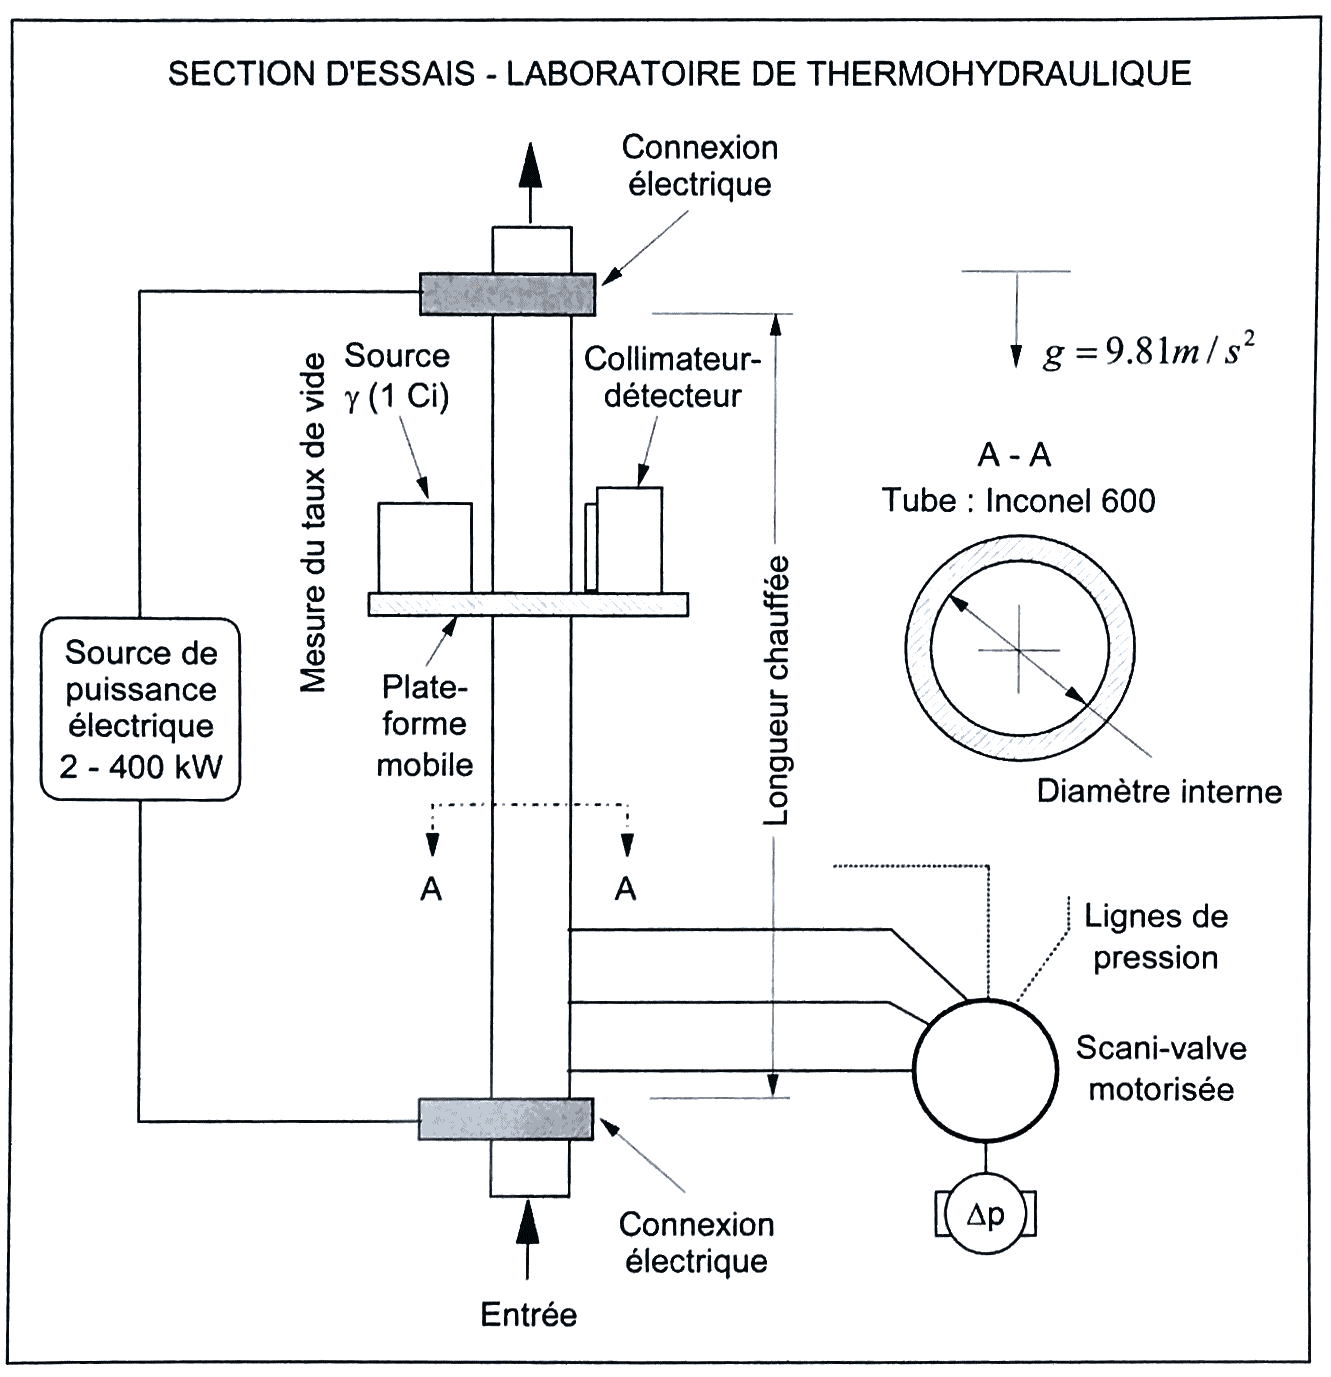
\includegraphics[width=0.7\textwidth]{images/schema_instal.png}
    \caption{Installation pour mesure de perte de pression et du taux de vide - D'après l'énoncé}
    \label{fig:instal}
\end{figure}

Le but de ce projet est de réaliser un modèle numérique et de déterminer les différents paramètres le long de la conduite. L'analyse des résultats se fait en comparant à des tables de données expérimentales. On travaille dans le cas d'un écoulement vertical ascendant.\\ \par
Pour réaliser cela, plusieurs hypothèses ont été réalisées :
\begin{itemize}
    \item \textbf{H1} : L'écoulement est incompressible.
    \item \textbf{H2} : La perte de pression par accélération dans la région non bouillante est négligeable.
    \item \textbf{H3} : La perte de pression totale est négligeable par rapport à la pression de l'écoulement.
    \item \textbf{H4} : L'enthalpie de l'eau sous-refroidie à une température donnée est égale à l'enthalpie de saturation de l'eau correspondant à cette température
\end{itemize}
\vspace{12pt}
\par
La détermination des propriétés thermodynamiques a été faite avec \texttt{pyXSteam}, qui est une librairie Python sur la base de \texttt{X-Steam} disponible sur Excel et Matlab.\\
Le titre et le taux de vide moyen sont déterminés à l'aide des corrélations de \textsc{Chexal-Lellouche} et de \textsc{Inoue}. Le multiplicateur diphasique ainsi que les facteurs de frottements qui servent au calcul de la perte de pression proviennent eux de la corrélation de \textsc{Friedel}.\\ \par






\newpage
%\section{Question 2\label{section:ex2}}

On considère l'écoulement d'un mélange diphasique dans un coude. On considère la section de l'écoulement constante. De plus, on fait implicitement l'hypothèse que l'écoulement est localement suivant la normale à chacune des sections de passage.\\

On rappelle les hypothèses suivantes :
\begin{itemize}
    \item \textbf{H1} : L'écoulement dans le coude est permanent (\textbf{H1.1}), uniforme (\textbf{H1.2}) et adiabatique (\textbf{H1.3})
    \item \textbf{H2} : On négligera les frottements en paroi (\textbf{H2.1}) ainsi que les forces volumiques (\textbf{H2.2})
     \item \textbf{H3} : La pression du gaz est égal à la pression du liquide : $P_L = P_G = P$
\end{itemize}

\subsection{Conservation de la masse}

En utilisant l'équation (8.5) des notes de cours :
\begin{equation}
    \overbrace{\cancel{\pder{\tau}{\rho_m}}}^{H1.1} + \pder{z}{G} = 0
\end{equation}

Soit un flux massique $G=cte$ le long du cylindre (fût-il courbe), que l'on réécrit en développant les termes :

\begin{equation}
    (1-\varepsilon_1)\rho_{L1}v_{L1} + \varepsilon_1 \rho_{G1}v_{G1} = (1-\varepsilon_2)\rho_{L2}v_{L2} + \varepsilon_2 \rho_{G2}v_{G2}
\end{equation}

On fait ici l'hypothèse que le coefficient de corrélation entre les quantités moyennées peut être pris égal à 1.

\subsection{Bilan de quantité de mouvement}

On effectue un bilan de quantité de mouvement sur le fluide contenu dans le coude, c'est-à-dire dans le volume délimité par les murs latéraux ainsi que les surfaces 1 (entrée) et 2 (sortie). \\

D'après l'hypothèse H1.1, la variation temporelle locale de quantité de mouvement dans le coude est nulle. On peut donc en conclure que l'ensemble des efforts extérieurs au système balance la différence de quantité de mouvement entre l'entrée et la sortie.\\

La quantité de mouvement entrante est égale à :
\begin{equation}
    \sum_{k=L,G} A\varepsilon_{1k}\rho_{1k} v_{1k}^2 \hat{j}
\end{equation}

Et de même pour celle sortante portée par $-\hat{i}$.\\

Les efforts extérieurs à prendre en compte  sont :

\begin{itemize}
    \item les forces de pression sur les faces entrantes et sortantes $A \left(P_1 \hat{j} - P_2 \hat{i}\right)$
    \item La force exercée par les parois du coude sur le fluide (qui sont des efforts de pression en paroi) $\vec{F}_{c\rightarrow f}$
    \item les frottements en parois qui sont négligés
    \item Le poids que l'on néglige
\end{itemize}

Finalement :
\begin{equation}
    -\sum_k A\varepsilon_{1k}\rho_{1k} v_{1k}^2 \hat{j} + \sum_k A\varepsilon_2\rho_{2k} v_{2k}^2 (-\hat{i}) = \vec{F}_{c\rightarrow f} + A\left( P_1 \hat{j} + P_2 \hat{i} \right) 
\end{equation}

En utilisant la conservation de la masse, on pourrait écrire plus simplement les efforts exercés par l'écoulement sur le coude $\vec{F}_{f\rightarrow c}$ en utilisant le volume spécifique de la quantité de mouvement. Néanmoins pour ne pas alourdir les notations, on conclura avec :

\begin{equation}
\boxed{
\begin{split}
        \vec{F}_{f\rightarrow c} = - \vec{F}_{c \rightarrow f} = & A\left[ \varepsilon_1\rho_{G1}v_{G1}^2 + (1-\varepsilon_1)\rho_{L1}v_{L1}^2 -P_1 \right] \hat{j} \\
          & +  A \left[\varepsilon_2 \rho_{G2}v_{G2}^2 + (1-\varepsilon_2)\rho_{L2}v_{L2}^2  - P_2 \right] \hat{i}
\end{split}
}
\end{equation}

%\newpage
%\section{Question 3\label{section:ex3}}

On se propose d'utiliser le modèle à écart de vitesse pour dériver un certain nombre de relations. La forme utilisée est la suivante :

\begin{equation}
    <u_g>_{2g} = <V_{gj}>_{2g} + C_0 <j>_2
\end{equation}

\subsection{Lien entre taux de vide $\varepsilon$ et fraction volumique $\beta$}

En écrivant la fraction volumique comme 
\begin{equation}
    \beta = \frac{<j_g>_2}{<j>_2} = \frac{<j_g>_2}{<j_g>_2 + <j_l>_2}
\end{equation}
avec $<j_g>_2 = \varepsilon<u_g>_{2g}$, on obtient :
\begin{equation}
    <u_g>_{2g} = \frac{\beta}{\varepsilon}<j>_2
\end{equation}

En injectant cette forme dans le modèle à écart de vitesse, on obtient :

\begin{equation}
\boxed{
    \frac{\beta}{\varepsilon} = \frac{<V_{gj}>_{2g}}{<j>_2} + C_0
    }
\end{equation}

\subsection{Expression pour le taux de vide moyen}

On fera l'hypothèse que le coefficient de corrélation entre masse volumique et vitesse pourra être pris égal à 1, comme cela a été fait dans la démarche présentée en cours. Notamment on prendre $<\rho_g u_g> = 1 \times <\rho_g><u_g> = \rho_g <u_g>$. A partir de cette hypothèse, on transforme l'expression de la vitesse superficielle :

\begin{equation}
    <j>_2 = \frac{G_g}{\rho_g} + \frac{G_l}{\rho_l} = G_l \left( \frac{1}{\rho_l} + \frac{1}{\rho_g} \frac{G_g}{G_l} \right)
\end{equation}

De même le premier terme dans le modèle à écart de vitesse est réécrit de telle sorte que l'on fait apparaître le flux massique de la phase liquide ainsi que le rapport $G_l/G_g$ :

\begin{equation}
    <u_g>_{2g} = \frac{G_l}{\varepsilon \rho_g}\frac{G_g}{G_l}
\end{equation}


Enfin en écrivant le titre de l'écoulement $\hat{x}$ comme 
\begin{equation}
    \hat{x} = \frac{1}{1 + \frac{G_l}{G_g}}
\end{equation}
Que l'on inverse en :

\begin{equation}
    \frac{G_g}{G_l} = \frac{\hat{x}}{1 - \hat{x}}
\end{equation}

En injectant ces développements dans le modèle à écart de vitesse on obtient:

\begin{equation}
    \underbrace{\frac{G_l}{\varepsilon \rho_g} \frac{\hat{x}}{1 - \hat{x}}}_{<u_g>_{2g}} = <V_{gj}>_{2g} + C_0 \times \underbrace{G_l \left( \frac{1}{\rho_l} + \frac{1}{\rho_g} \frac{\hat{x}}{1 - \hat{x}}\right)}_{<j>_2}
\end{equation}

Enfin on isole le taux de vide : 

\begin{equation}
\boxed{
    \frac{1}{\varepsilon} = \frac{\rho_g}{G_l} \frac{1 - \hat{x}}{\hat{x}}<V_{gj}>_{2g} + C_0\left( \frac{\rho_g}{\rho_l}\frac{1-\hat{x}}{\hat{x}} + 1\right) 
    }
\end{equation}

\subsection{Comparaison avec les résultats expérimentaux}

Pour rappel, d'après l'équation (13.87) des notes de cours, on a égalité des titres de l'écoulement et thermodynamique lors d'un mélange liquide-vapeur à saturation, ce qui est le cas ici. \\

Le code python est proposé en annexe. Les valeurs numériques des données expérimentales ont été récupérées en utilisant \verb|Web Plot Digitizer|. On se référera à la figure \ref{fig:Pb3CompExperiment} pour les résultats. Les modèles analytiques ont été tracés pour des valeurs du titre strictement positives. \\

On remarque que le choix dans le modèle de corrélation joue un rôle significatif. En effet on obtient un accord expériences-modèle plutôt bon avec la corrélation de Inoue, au moins pour les valeurs de $G$ faibles (en pratique $G\lesssim 250$). En revanche la corrélation de Maier semble donner de moins bons résultats.


\begin{figure}
    \centering
    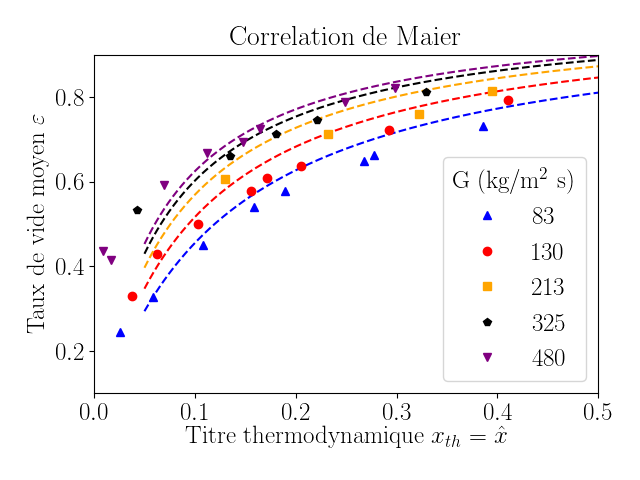
\includegraphics[width=0.47\linewidth]{images/MaierCorrelation.png}
    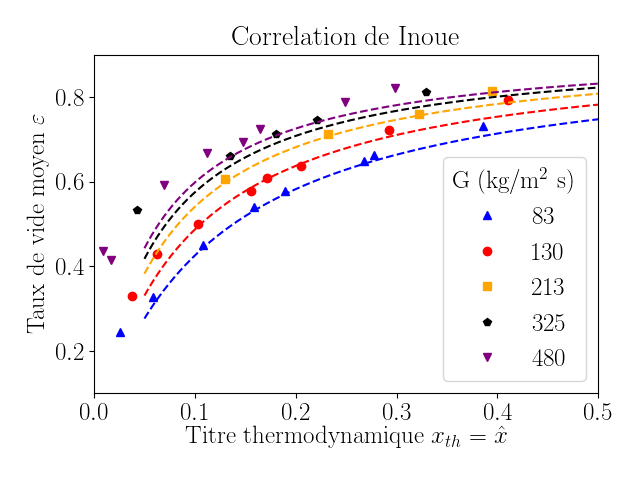
\includegraphics[width=0.47\linewidth]{images/InoueCorrelation.png}
    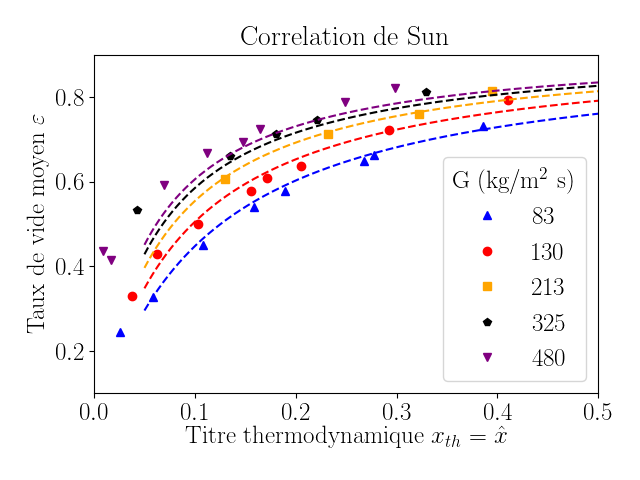
\includegraphics[width=0.47\linewidth]{images/SunCorrelation.png}
    \caption{Comparaison des corrélations de (Maier \& Coddigton, 1997), (Inoue \& al, 1993) et (Sun \& al, 1980) avec les données expérimentales de (Zuber \& al, 1967)}
    \label{fig:Pb3CompExperiment}
\end{figure}
%\newpage
%\section{Question 4\label{section:ex4}}


\colorlet{droplet color}{blue!50!cyan!80}
\tikzset{%
  raindrop/.pic={
    code={\tikzset{scale=1/10}
 \shade [shading=droplet]
 (0,0)  .. controls ++(0,-1) and ++(0,1) .. (1,-2)
 arc (360:180:1)
 .. controls ++(0,1) and ++(0,-1) .. (0,0) -- cycle;
  }}}

\begin{figure}[H]
\begin{center}
\begin{tikzpicture}[line join=round,rotate=270]
\filldraw[draw=black,ultra thick,fill=droplet color!20]
 (0,12) arc[x radius=2, y radius=0.4, start angle=180, end angle=0]
 (4,12) arc[x radius=2, y radius=0.4, start angle=0, end angle=-180];
\filldraw[ultra thick,fill=droplet color!70,opacity=1,fill opacity=0.7]
  (0,12) -- 
  (0,0) 
  arc[x radius=2, y radius=0.4, start angle=-180, end angle=0] --
   (4,12)
  arc[x radius=2, y radius=0.4, start angle=0, end angle=-180];
\draw[dashed] 
  (0,0) arc[x radius=2, y radius=0.4, start angle=180, end angle=0];

%\draw[red,<->, thick] (0,9) -- (1,9)node[right] {$R$}-- (2,9);
\draw[black,->,dotted] (-1.5,1.5) -- (-0.05,1);
\draw[black,->,dotted] (-1.5,3.5) -- (-0.05,3);
\draw[black,->,dotted] (-1.5,5.5) -- (-0.05,5);
\draw[black,->,dotted] (-1.5,7.5) -- (-0.05,7);
\draw[black,->,dotted] (-1.5,9.5) -- (-0.05,9);
\draw[black,->,dotted] (-1.5,11.5)node[above left]{$P = 150 \si{kW}$} -- (-0.05,11);

\draw[black,->,dotted] (5.5,1.5) -- (4.05,1);
\draw[black,->,dotted] (5.5,3.5) -- (4.05,3);
\draw[black,->,dotted] (5.5,5.5) -- (4.05,5);
\draw[black,->,dotted] (5.5,7.5) -- (4.05,7);
\draw[black,->,dotted] (5.5,9.5) -- (4.05,9);
\draw[black,->,dotted] (5.5,11.5) -- (4.05,11);

\draw[black,->,thick] (1,-1.5) -- (1,-0.5);
\draw[black,->,thick] (2,-1.5)node[left]{Inlet} -- (2,-0.5);
\draw[black,->,thick] (3,-1.5) -- (3,-0.5);

\draw [thick,red] [<->] (0,13) --++(2,0) node [right] {$\varnothing = 13,3 \si{mm}$} --++(2,0);
\draw [thick] [<->] (6,0) --++(0,6) node [below] {$L=1,90 \si{m} $}--++(0,6);
%\draw [thick] [->] (1,10.5) --++(-0.5,-0.4) node [below left]
%{$\vec{e_{\theta}}$};
%\draw[dashed] (2,9.9)--(1.5,10.2)node [right]{$r$}-- (1,10.5);


%\draw[black,dotted, thick] (0,2) -- (4,2);
%\draw[black,dotted, thick] (0, 2) .. controls(1,4) and (3,4) .. (4, 2);
%\draw[black,->, thick] (1,2) -- (1,3.1);
%\draw[black,->, thick] (3,2) -- (3,3.1);
%\draw[black,->, thick] (2,2) -- (2,3)node[below] {$\vec{u}$} -- (2,3.5);
%\draw[black,->, thick]    (2.5,3) -- (2.5,4)node[below] {$\dot{Q}_G = 0,002$ \si{m^3/s}} -- (2.5,5);
\end{tikzpicture}

\caption{Schéma de la conduite pour étudier la chute de pression}
    \label{fig:ConfigExo4}
    \end{center}
\end{figure}

Dans cet exercice, nous travaillons avec une conduite chauffée uniformément par une puissance $P = 150 \si{kW}$ comme représentée sur la fig. \ref{fig:ConfigExo4}. Les paramètres à l'entrée de la conduite (noté Inlet sur le schéma) sont donnés comme :

\begin{equation}
    \left\{
    \begin{array}{r c l l}
    P &=& 30 & \si{bar} \\
    T_{SR} &=& 10 & \si{K}\\
    \dot{m} &=& 0.42 &\si{kg/s}
    \end{array}
    \right.
\end{equation}
\\
On rappelle les hypothèses utilisés dans ce problème :
\begin{itemize}
    \item \textbf{H1} : L'écoulement est incompressible.
    \item \textbf{H2} : La perte de pression par accélération dans la région non bouillante est négligeable.
     \item \textbf{H3} : La perte de pression totale est négligeable par rapport à la pression de l'écoulement.
\end{itemize}
\vspace{12pt}
\par
\subsection{Titre thernodynamique nul - $x$}
Comme il y a une température de sous-refroidissement $T_{SR}$ en entrée, la température de saturation de l'eau à 30 \si{bar} (qui est égale à 233,7\degre C) n'est atteinte que plus loin dans la conduite. On cherche donc la distance qu'il faut pour réchauffer l'écoulement de 10 \si{K}, qui correspond à l'endroit où le titre thermodynamique est nul.
On peut écrire :
\begin{equation}
    \dot{Q}_{sat} = \dot{m} Cp \Delta T
\end{equation}
Le terme $Cp$ pouvant être pris pour une pression de 30 \si{bar}, il vaut alors 4715,9 \si{kJ/kg K}. On a trouve alors que la puissance nécessaire est de :
\begin{equation}
    P_{sat} = 19.8 \si{kW}
\end{equation}
Comme on considère que la conduite est chauffée uniformément, le rapport entre puissance nécessaire pour arriver à saturation et puissance totale thermique ajoutée $P_{th}$ est égale au rapport entre $L_{sat}$ et longueur totale chauffée $L_c$. on a alors :
\begin{equation}
\boxed{
    L_{sat}= \frac{ P_{sat}\times L_c}{P_{th}} = \frac{19.8 \times 1,9}{150} = 0.25~\si{m} 
    }
\end{equation}
\subsection{Titre thermodynamique en sortie - $x_s$}
Nous pouvons donc maintenant nous concentrer sur l'obtention du titre en sortie de la conduite.\\
La conservation de l'énergie nous donne la forme suivante pour le titre :
\begin{equation}
    x_s = \frac{4}{G}\frac{1}{D}\frac{q''}{h_{lv,sat}}L
\end{equation}
Cette forme est valable à partir du moment où le titre est nul. Dans notre cas, la conduite ne fait donc plus L = 1.9 \si{m} mais il faut lui enlever la région non-bouillante qui fait 0.25 \si{m}.\\ \par
Définissons maintenant les termes que nous avons besoin pour cette équation. Commençons par les surfaces, il y a la surface de la paroi et la section de la conduite qui donnent respectivement :
\begin{equation}
    S_{par} = L_c \times \pi D = \num{0.0794}~\si{m^2}
\end{equation}

\begin{equation}
    S_{con} = \frac{\pi D^2}{4} = \num{1.3894e-4}~\si{m^2}
\end{equation}
On peut ainsi définir le flux massique $G$ :
\begin{equation}
    G = \frac{\dot{m}}{S_{con}} = \num{3023.13} ~\si{kg/m^2s}
\end{equation}
Et $q''$ le flux de chaleur sur la paroi :
\begin{equation}
    q'' = \frac{P}{S_{par}} = \num{1889,5} ~\si{kW/m^2}
\end{equation}

Enfin le dernier terme nécessaire est $h_{lv,sat}$ qui est la différence entre l'enthalpie à saturation du gaz et du liquide :
\begin{equation}
    h_{lv,sat} = h_{v,sat} - h_{l,sat} = 2803 -1007,7 = 1795,3 ~\si{kJ/kg}
\end{equation}
Les valeurs proviennent des tables de saturation de l'eau à une pression de 30 \si{bar}.\\
On a alors : 
\begin{equation}\boxed{
    x_s = \frac{4}{G}\frac{1}{D}\frac{q''}{h_{lv,sat}} \left(L_c - L_{sat}\right) = 0,173
    }
\end{equation}
\subsection{Perte de pression totale - $\Delta P$}

On peut désormais s'intéresser à la perte de pression dans la conduite qui est de la forme : 
\begin{equation}
\begin{array}{c}
-\Delta P=\frac{1}{2} f \frac{G^{2}}{\rho_{l}} \frac{L}{D} \overbrace{\left[\frac{1}{x_{e}} \int_{0}^{x_{e}} \phi_{l_{0}}^{2} d x\right]}^{\text{Multiplicateur diphasique}}+\frac{G^{2}}{\rho_{l}}\overbrace{\left[\frac{x_{e}^{2}}{\varepsilon_{e}} \frac{\rho_{l}}{\rho_{v}}+\frac{\left(1-x_{e}\right)^{2}}{\left(1-\varepsilon_{e}\right)}-1\right]}^{\Delta P\text{ par accélération}} \\
+\underbrace{\cancel{\frac{L}{x_{e}} g \int_{0}^{x_{e}}\left[\rho_{v} \varepsilon+\rho_{l}(1-\varepsilon)\right] d x}}_{\text{Conduite horizontale $g=0$}}
\end{array}
\end{equation}

Les termes du \og Multiplicateur diphasique \fg{} et \og Perte de pression par accélération \fg{} sont obtenus par lecture dans des abaques. On peut alors, avec le titre en sortie $x_s=17,3\%$ et $P = 30 ~ \si{bar}$ , en déduire :
\begin{equation}
    \left\{
    \begin{array}{r c l}
    \left[\frac{1}{x_{e}} \int_{0}^{x_{e}} \phi_{l_{0}}^{2} d x\right] &=& 8 \\[2ex]
    \left[\frac{x_{e}^{2}}{\varepsilon_{e}} \frac{\rho_{l}}{\rho_{v}}+\frac{\left(1-x_{e}\right)^{2}}{\left(1-\varepsilon_{e}\right)}-1\right] &=& 4 \\
    \end{array}
    \right.    
\end{equation}
Le terme  noté $f$, correspond au facteur de frottement monophasique, défini comme :
\begin{equation}
    f=0.316\left[\text{Re}_L \right]^{-0.25} = 0.316\left[\frac{(1-x) G D}{\mu_l} \right]^{-0.25}
\end{equation}
%La vitesse moyenne de la phase liquide de l'écoulement se détermine avec le %débit massique :
%\begin{equation}
%    u_l = \frac{\dot{m}}{\rho_l}\frac{1}{S_{con}} = 3.67~ \si{m/s}
%\end{equation}
Et en utilisant les valeurs :
\begin{equation}
    \left\{
    \begin{array}{r c l l}
%    \rho_l &=& 823.1 &\si{kg/m^3}\\
    x &=& 0.173 & \\
    \mu_l &=& \num{116,4e-6} &\si{Pa.s}
    \end{array}
    \right.    
\end{equation}
Nous obtenons, $\text{Re}_L = \num{287493,7}$ soit $f = \num{0,0136}$\\

En injectant le tout dans l'équation de la perte de pression on obtient :
\begin{equation}
    \boxed{
    -\Delta P = \num{130709} ~\si{Pa} = 1.31 ~\si{bar}
    }
\end{equation}
%\newpage
%\section*{Annexes\label{section:annexes}}


\subsection*{Code utilisé pour le problème 3}

{
\scriptsize
\inputminted[
frame=lines,
framesep=2mm,
baselinestretch=1,
linenos
]{python}{Pb3.py}

}

% References
%\bibliographystyle{plain}
%\bibliography{references}
\end{document}
